\chapter{Progettazione della Soluzione}
\section{Class Diagram del dominio della soluzione}
	\begin{figure}[hbt]
	\centering
  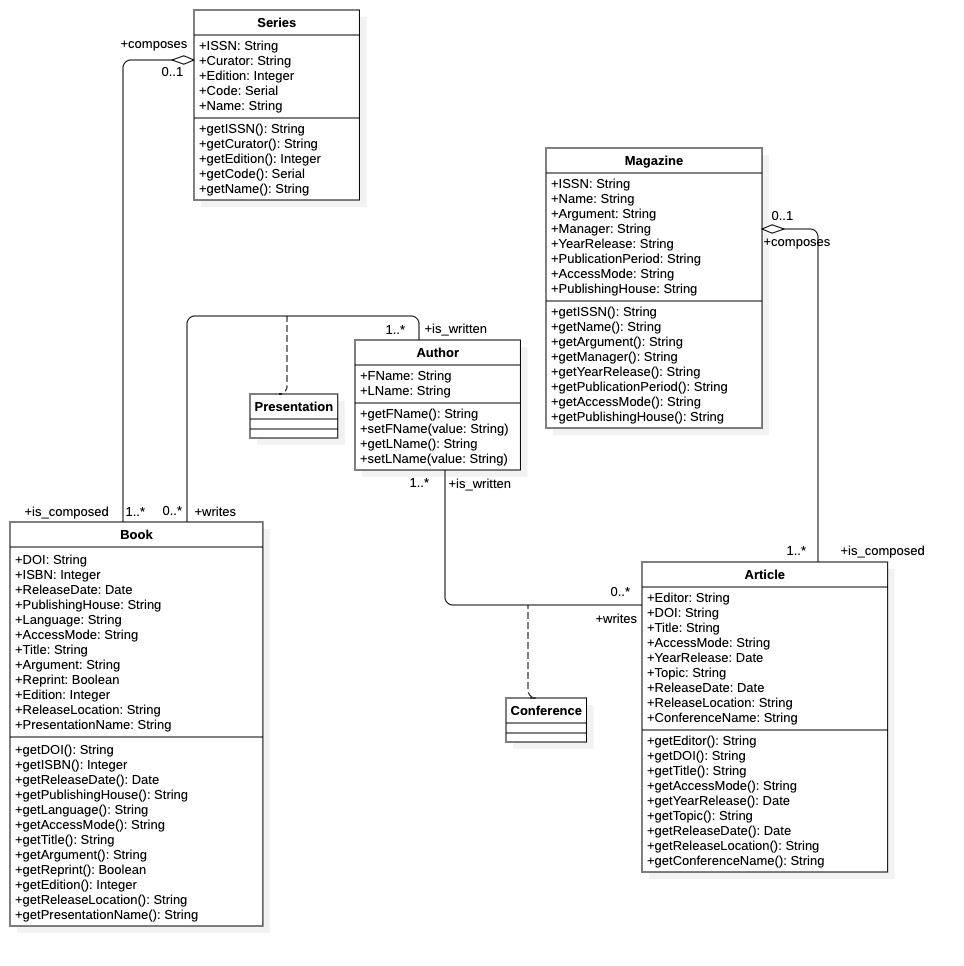
\includegraphics[width=0.9\textwidth]{/Users/lorenzotecchia/Documents/ESAMI/ProgettoOOBD/OO/Documentazione/Diagrammi/CD_DS.png}
  \caption{Class Diagram del dominio della soluzione}
\end{figure}


% Please add the following required packages to your document preamble:
% \usepackage{longtable}
% Note: It may be necessary to compile the document several times to get a multi-page table to line up properly
\begin{longtable}[c]{|l|l|}
\caption{Dizionario dei Metodi}
\label{tab:DIzionarioMetodi}\\
\hline
\rowcolor[HTML]{E5150C} 
 Classe & Metodi                                                                                                                                                                                                                                                                                                                                                                       \\ \hline
\endhead
%
Series                                              & \begin{tabular}[c]{@{}l@{}}+getISSN(): String\\  +getCurator(): String\\  +getEdition(): Integer\\  +getCode(): Serial\\ +getName(): String\end{tabular}                                                                                                                                                                                                                     \\ \hline
Author                                              & \begin{tabular}[c]{@{}l@{}}+getFName(): String\\ +getLName(): String\end{tabular}                                                                                                                                                                                                                                                                                            \\ \hline
Magazine                                            & \begin{tabular}[c]{@{}l@{}}+getISSN():String\\ +getName(): String\\ +getArgument(): String\\ +getManager(): String\\ +getYearRelease: Timestamp\\  +getPublicationPeriod(): String\\  +getAccessMode(): String\\  +getPublishingHouse(): String\end{tabular}                                                                                                                 \\ \hline
Article                                             & \begin{tabular}[c]{@{}l@{}}+getEditor(): String \\ +getDOI(): String\\  +getTitle(): String\\  +getAccessMode(): String   \\ +getTopic(): String \\  +getReleaseDate(): Timestamp  \\ +getReleaseLocation(): String  \\  +getConferenceName(): String\end{tabular}                                                                                                           \\ \hline
Book                                                & \begin{tabular}[c]{@{}l@{}}+getDOI0: String \\ +getISBN(): Integer \\ +getReleaseDate(): Date  \\ +getPublishingHouse(): String  \\ +getLanguage(): String  \\ +getAccessMode(): String \\ +getTitle(): String \\ +getArgument(): String \\ +getReprint(): Boolean \\ +getEdition(): Integer \\ +getReleaseLocation(): String \\ +getPresentationName(): String\end{tabular} \\ \hline
Presentation                                        & \begin{tabular}[c]{@{}l@{}}+getTitle() \\ +getFirstname() \\ +getLastname() \\ +getConferenceName() \\ +getReleaseLocation() \\ +getReleasedate()\end{tabular}                                                                                                                                                                                                               \\ \hline
Conference                                          & \begin{tabular}[c]{@{}l@{}}+getTitle() \\ +getFirstname() \\ +getLastname() \\ +getConferenceName() \\ +getReleaseLocation() \\ +getReleasedate()\end{tabular}                                                                                                                                                                                                               \\ \hline
\end{longtable}
	\newpage
	\section{Sequence Diagram del metodo ReadAllBooks}
	\begin{figure}[hbt]
  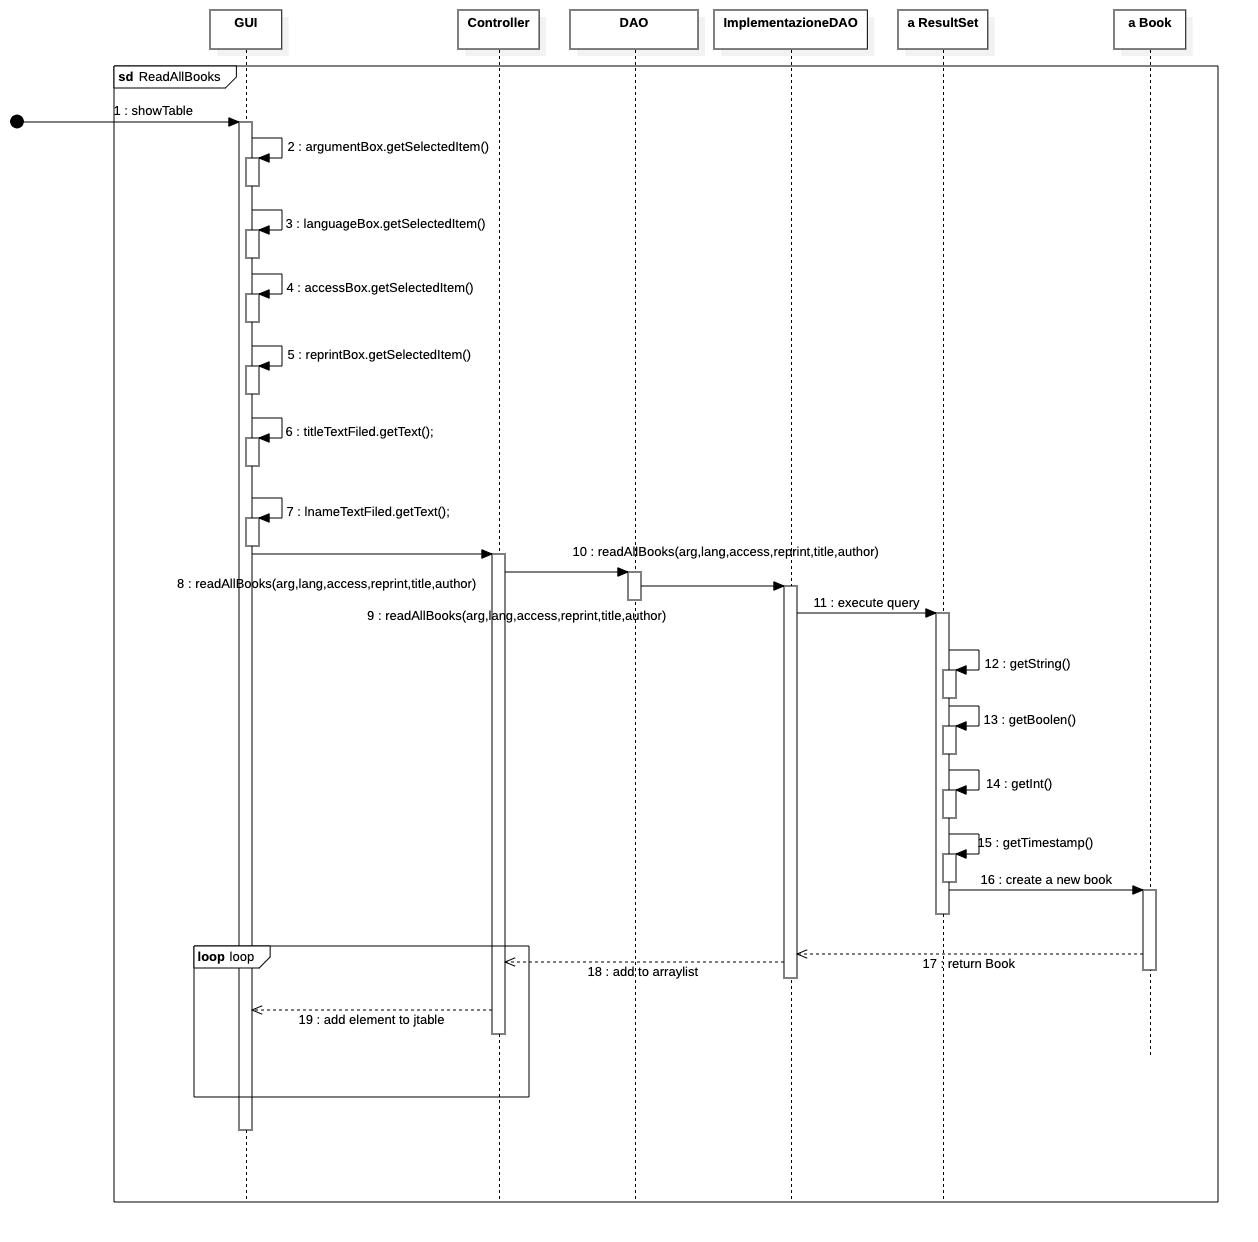
\includegraphics[width=\textwidth]{Immagini/ReadAllBooksSD.png}
  \caption{Sequence Diagram per il metodo della gui per la visualizzazione dei libri}
\end{figure}
\newpage

	\section{Sequence Diagram del metodo getAllArgumentsBooks}
	\begin{figure}[hbt]
  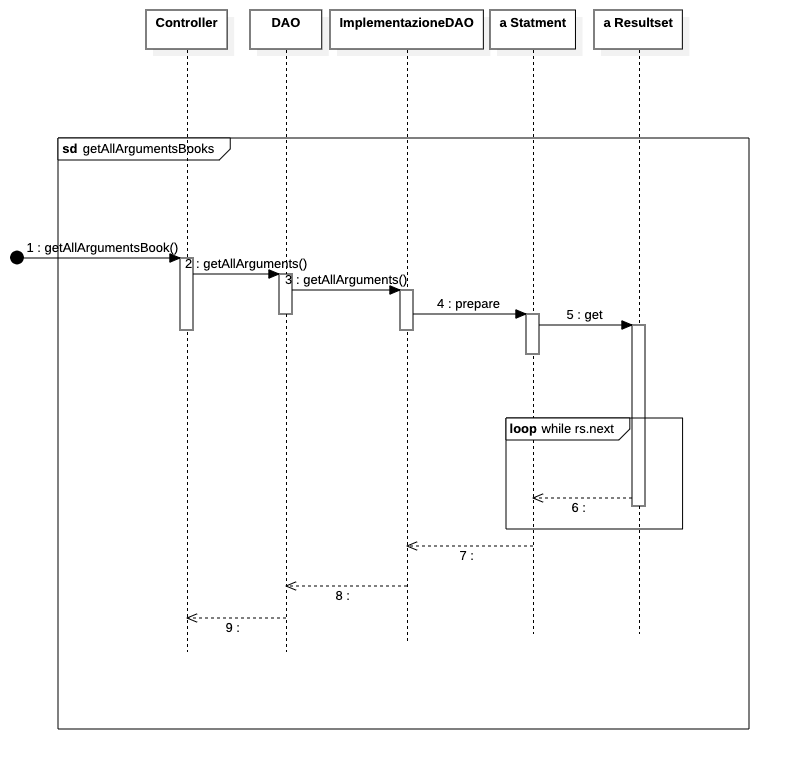
\includegraphics[width=\textwidth]{Immagini/getAllArgumentsBooksSD.png}
  \caption{Sequence diagram per il metodo di ritorno di tutti gli argomenti di un libro}
\end{figure}
